\chapter{Pembuatan Model Termal Satelit LAPAN-A3}

Bab ini akan membahas langkah-langkah untuk membuat model termal semi-empiris
satelit LAPAN-A3 menggunakan metode \textit{machine learning}. Diagram alir
proses pembuatan model termal tersebut dapat dilihat kembali pada Gambar
\ref{fig:metodologi} yang memuat metodologi penelitan pada karya tulis ini
secara umum. Kemudian, karena persamaan-persamaan terkait perhitungan variabel
model termal sudah dibahas secara menyeluruh pada bab Tinjauan Pustaka, bab ini
hanya akan membahas bagaimana variabel pada persamaan-persamaan tersebut dapat
dihitung dari data yang sudah dikumpulkan. Penjabaran fungsi dan algoritma
dalam pembuatan model termal lebih mendalam dapat dilihat di kode sumber
pemrograman karya tulis ini yang tersedia di repositori
https://github.com/sutricky/a3thermalmodel pada situs \textit{Github}.

\section{Pengumpulan Data}

Data untuk penelitian di karya tulis ini dapat dibagi menjadi 2 jenis : data
telemetri satelit LAPAN-A3 serta data \textit{two-line elements} (TLE). Data
telemetri satelit LAPAN-A3 diperoleh dari data operasional internal LAPAN,
sedangkan data TLE LAPAN-A3 diambil dari situs Celestrak \cite{kelso}. Kedua
jenis data dikumpulkan untuk periode observasi 19 sampai dengan 20 Mei 2018.
Contoh data telemetri satelit LAPAN-A3 dapat dilihat pada Gambar
\ref{fig:telea3} dan contoh data TLE LAPAN-A3 dapat dilihat pada Gambar
\ref{fig:tlea3}.

\begin{figure}[H]
\setlength\belowcaptionskip{-0.7\baselineskip}
\begin{center}
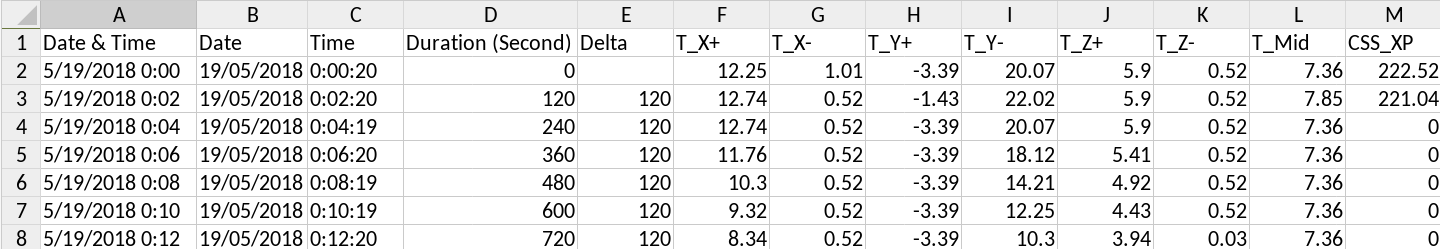
\includegraphics[width=0.8\textwidth]{fig/telea3.png}
\caption{Contoh data telemetri LAPAN-A3}
\label{fig:telea3}
\end{center}
\end{figure}

\begin{figure}[H]
\setlength\belowcaptionskip{-0.7\baselineskip}
\begin{center}
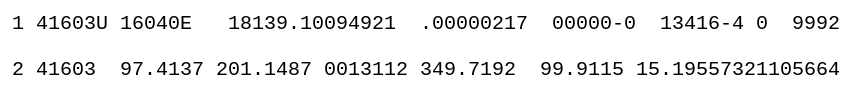
\includegraphics[width=0.7\textwidth]{fig/tlea3.png}
\caption{Contoh data TLE LAPAN-A3}
\label{fig:tlea3}
\end{center}
\end{figure}

Data telemetri satelit LAPAN-A3 yang dibutuhkan mencakup pembacaan sensor suhu
dan sinar Matahari \textit{node-node} satelit serta sikap satelit selama
periode observasi. Sesuai dengan model satelit LAPAN-A3 yang digunakan, data
yang disediakan oleh LAPAN juga sudah berupa bacaan sensor dari 6 sisi satelit
dan plat tengah satelit.

Selanjutnya, nilai TLE satelit diasumsikan tidak berubah selama 1 periode
observasi. Karena itu, \textit{epoch} atau waktu acuan yang digunakan untuk
perhitungan orbit satelit selama 1 hari pada bagian berikutnya adalah data TLE
pertama yang tersedia pada periode observasi sesuai zona waktu UTC. Asumsi ini
didasari oleh algoritma SGP-4 yang digunakan untuk mempropagasi orbit satelit
LAPAN-A3 memiliki akurasi yang cukup untuk memprediksi orbit satelit dalam
rentang waktu 15 hari dari waktu acuan \cite{kelsoa}. Secara spesifik untuk
LAPAN-A3, selisih kesalahan rata-rata perhitungan posisi LAPAN-A3 yang
menggunakan data TLE terbaru dan data TLE 1 hari sebelumnya bernilai 0.364 km
\cite{nugroho2018}. 

\section{Pembuatan Dataset}

Sebagai gambaran umum, diagram alir yang ditunjukkan Gambar \ref{fig:algoritma}
pada bagian Metodologi memperlihatkan \textit{pipeline} data dalam pembuatan
dataset untuk model \textit{machine learning}. Pembuatan dataset dilakukan
dengan mempersiapkan dataset dasar, menghitung faktor termal satelit, dan
menyaring dataset.

\subsection{Persiapan Dataset Dasar}

Data mentah yang sudah dikumpulkan di tahap sebelumnya diproses terlebih dahulu
lewat kode Python sehingga memiliki bentuk dan satuan yang sesuai untuk
diproses lebih lanjut di tahap berikutnya. Proses ini dilakukan hanya pada data
mentah telemetri satelit LAPAN-A3 karena data TLE sudah dalam format yang dapat
digunakan oleh modul Skyfield. Secara singkat, data bacaan sensor suhu
\textit{node} satelit diubah menjadi satuan K, bacaan arus pada sensor Matahari
menjadi satuan A, dan sikap satelit menjadi satuan rad. Selain itu, data
perubahan suhu \textit{node} satelit antar selang waktu observasi juga turut
dihitung. Kemudian, data waktu pembacaan sensor-sensor satelit dipisah menjadi
format tahun, bulan, tanggal, jam, menit, dan detik untuk memudahkan propagasi
orbit di bagian berikutnya. Gambar \ref{fig:basedataset} menunjukkan
contoh dataset dasar yang dihasilkan dari kode Python.

\begin{figure}[H]
\setlength\belowcaptionskip{-0.7\baselineskip}
\begin{center}
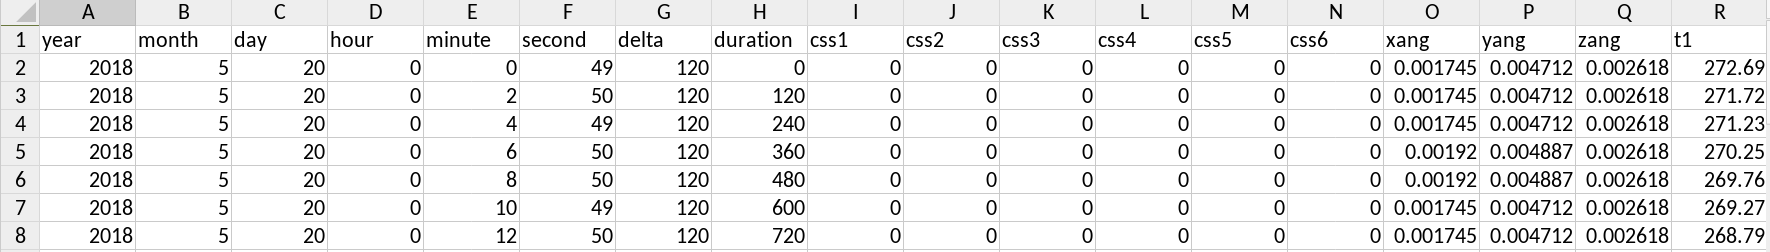
\includegraphics[width=0.8\textwidth]{fig/basedataset.png}
\caption{Contoh dataset dasar keluaran kode Python}
\label{fig:basedataset}
\end{center}
\end{figure}

\subsection{Perhitungan Faktor Termal Satelit}

Sesuai diagram alir \textit{pipeline} yang ditunjukkan Gambar
\ref{fig:algoritma} dan tabel variabel yang masih belum diketahui pada Tabel
\ref{table:unknown}, perhitungan faktor termal satelit terbagi mencakup 3 jenis
variabel : faktor panas akibat Matahari, Bumi, dan albedo. Ketiga jenis
variabel tersebut dihitung juga menggunakan kode Python. 

Pertama, faktor panas akibat Matahari merupakan hasil perkalian bacaan arus
sensor Matahari \textit{node} dan faktor gerhana \textit{node} satelit. Sejalan
dengan definisi faktor gerhana node yang dijelaskan pada bab Tinjauan Pustaka,
nilai variabel tersebut dapat ditentukan dari pembacaan arus sensor sinar
Matahari \textit{node} terkait; bacaan arus lebih besar dari 0 A berarti
\textit{node} menerima sinar Matahari sehingga memiliki nilai faktor gerhana
sebesar 1. Sebaliknya, jika bacaan arus sensor \textit{node} bernilai 0,
\textit{node} tidak menerima sinar Matahari sehingga memiliki nilai faktor
gerhana 0.

Perhitungan faktor gerhana \textit{node} dari data arus sensor Matahari
\textit{node} harus memperhatikan toleransi kesalahan bacaan sensor yang
mungkin terjadi. Sebagai contoh, sensor Matahari pada satelit LAPAN-A3 yang
digunakan dalam karya tulis ini menunjukkan pembacaan lebih besar dari 0 A pada
beberapa selang waktu pengamatan meskipun seharusnya satelit berada pada fase
gerhana merujuk pada nilai bacaan arus sensor \textit{node} sebelum dan
sesudahnya. Bacaan arus sensor Matahari \textit{node} tersebut dapat dianggap
kesalahan pengukuran karena terjadi konsisten pada setiap sensor dengan besar
yang sama dan hanya terjadi pada beberapa selang waktu tertentu saat satelit
jelas dalam fase gerhana. Gambar \ref{fig:solarfactor} menunjukkan contoh hasil perhitungan faktor panas akibat Matahari. 

\begin{figure}[H]
\setlength\belowcaptionskip{-0.7\baselineskip}
\begin{center}
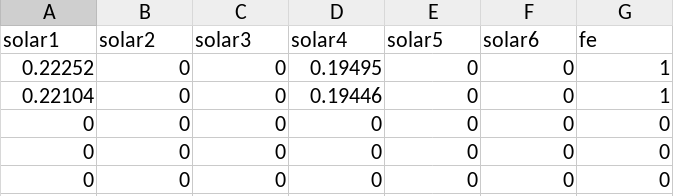
\includegraphics[width=0.6\textwidth]{fig/solarfactor.png}
\caption{Contoh hasil perhitungan faktor panas akibat Matahari}
\label{fig:solarfactor}
\end{center}
\end{figure}

Selanjutnya, faktor panas akibat Bumi dan albedo sama-sama bergantung pada
perhitungan \textit{view factor} \textit{node} satelit ke Bumi. Sesuai dengan
Persamaan \ref{eq:vf}, \textit{view factor} dari \textit{node} satelit ke Bumi
didekati dengan \textit{view factor} dari plat persegi panjang ke bola. Persamaan \ref{eq:vf} membutuhkan jari-jari bola $r$, jarak antara plat dengan bola $R$, dan sudut antara garis normal permukaan plat dengan garis jarak antara plat dan bola $\gamma$. 

Jari-jari bola $r$ dapat didekati dengan nilai rata-rata jari-jari Bumi sebesar
6371 km \cite{moritz}. Lalu, karena ukuran satelit jauh lebih kecil dari Bumi,
jarak plat ke bola $H$ dapat didekati dengan jarak antara satelit dan Bumi yang
dapat dihitung dengan mempropagasi orbit satelit berdasarkan data TLE
menggunakan modul Skyfield. Propagasi orbit lewat modul Skyfield juga
memungkinkan perhitungan vektor posisi satelit seiring perubahan waktu. Dengan
demikian, sudut antara garis normal permukaan plat dengan bola $\gamma$ dapat
didekati dengan sudut antara vektor normal permukaan \textit{node} dengan
vektor posisi satelit terhadap Bumi. 

Perhitungan sudut $\gamma$ perlu memperhatikan tata acuan koordinat yang
digunakan pada kedua vektor. Pada perhitungan \textit{view factor node} di
karya tulis ini, sistem koordinat yang digunakan adalah sistem koordinat bawaan
modul Skyfield yaitu \textit{Geocentric Celestial Reference System} (GCRS).
Karena itu, vektor normal permukaan \textit{node} harus dikonversi terlebih
dahulu dengan bantuan matriks rotasi sudut Euler dengan urutan Z-Y-X. Gambar
\ref{fig:vffig} menunjukkan contoh hasil perhitungan \textit{view factor node}
satelit ke Bumi dan Gambar \ref{fig:earthfactor} menunjukkan contoh hasil perhitungan faktor panas akibat Bumi.

\begin{figure}[H]
\setlength\belowcaptionskip{-0.7\baselineskip}
\begin{center}
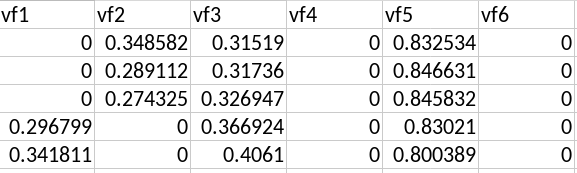
\includegraphics[width=0.6\textwidth]{fig/vffig.png}
\caption{Contoh hasil perhitungan \textit{view factor node} satelit ke Bumi}
\label{fig:vffig}
\end{center}
\end{figure}

\begin{figure}[H]
\setlength\belowcaptionskip{-0.7\baselineskip}
\begin{center}
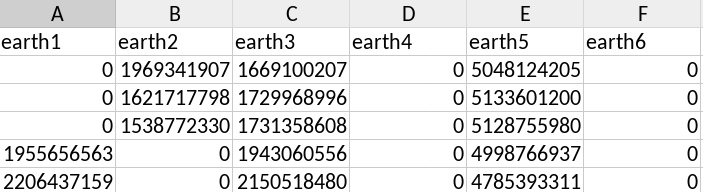
\includegraphics[width=0.6\textwidth]{fig/earthfactor.png}
\caption{Contoh hasil perhitungan faktor panas akibat Bumi}
\label{fig:earthfactor}
\end{center}
\end{figure}

Terakhir, perhitungan faktor panas akibat albedo juga membutuhkan faktor albedo
satelit. Sesuai dengan Persamaan \ref{eq:albedofactor}, nilai faktor albedo
satelit bergantung pada faktor gerhana satelit serta posisi sudut satelit dan
mulainya fase gerhana terhadap titik \textit{sub-solar}. Sama dengan
perhitungan faktor gerhana \textit{node}, faktor gerhana satelit akan bernilai
1 saat satelit menerima sinar Matahari dan bernilai 0 saat satelit berada pada
fase gerhana. Dengan demikian, faktor gerhana satelit bernilai 0 saat semua
\textit{node} satelit memiliki faktor gerhana 0 dan bernilai 1 jika ada 1 atau
lebih \textit{node} yang memiliki faktor gerhana 1.

Untuk mencari posisi sudut satelit dan mulainya fase gerhana terhadap titik
\textit{sub-solar}, perlu dihitung terlebih dahulu nilai anomali benar satelit
fase gerhana mulai dan berakhir. Nilai anomali benar satelit dapat dicari lewat
propagasi orbit menggunakan modul Skyfield berdasarkan data TLE sesuai data
waktu satelit dari data telemetri satelit. Dengan mengasumsikan simetri orbit
lingkaran sehingga titik \textit{sub-solar} berada di tengah titik akhir dan mulai fase gerhana satelit seperti yang ditunjukkan lokasi \textit{conjunction point} pada Gambar \ref{fig:ssp}, anomali benar titik \textit{sub-solar} dapat dihitung.

\begin{figure}[H]
\setlength\belowcaptionskip{-0.7\baselineskip}
\begin{center}
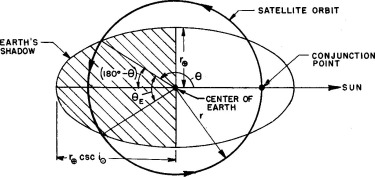
\includegraphics[width=0.6\textwidth]{fig/ssp.jpg}
	\caption[Ilustrasi fase gerhana pada orbit satelit]{Ilustrasi fase gerhana pada orbit satelit~\cite{ismail2015}}
\label{fig:ssp}
\end{center}
\end{figure}

Selanjutnya, posisi sudut satelit terhadap titik \textit{sub-solar} untuk waktu
tertentu dapat dicari dengan mengurangi anomali benar satelit dengan anomali
benar titik \textit{sub-solar}. Gambar \ref{fig:albedofactor} menunjukkan
contoh hasil perhitungan faktor panas akibat albedo.

\begin{figure}[H]
\setlength\belowcaptionskip{-0.7\baselineskip}
\begin{center}
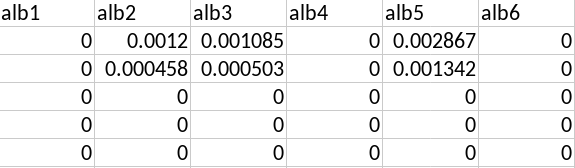
\includegraphics[width=0.6\textwidth]{fig/albedofactor.png}
\caption{Contoh hasil perhitungan faktor panas akibat albedo}
\label{fig:albedofactor}
\end{center}
\end{figure}

Karena \textit{node} 7 pada model satelit LAPAN-A3 mewakili plat tengah satelit
yang diasumsikan terisolasi dari lingkungan luar satelit, laju perubahan suhu
\textit{node} 7 dianggap tidak dipengaruhi faktor panas akibat Matahari,
albedo, maupun Bumi. Diasumsikan juga \textit{node} 7 tidak mengalami disipasi
panas ke lingkungan ruang angkasa sehingga perubahan suhu pada \textit{node} 7
murni terjadi akibat perpindahan panas lewat konduksi dan radiasi dengan
ke-enam \textit{node} lainnya.

\subsection{Penyaringan dataset}

Data gabungan dataset dasar dan hasil perhitungan koefisien faktor termal
satelit kemudian disaring untuk meminimalkan kesalahan dan menghilangkan
\textit{outlier} pembacaan sensor satelit. Kriteria yang digunakan untuk
menyaring dataset adalah sebagai berikut :

\begin{enumerate}
\item Selang waktu antar pengamatan maksimal 120 s 
\item Skor standar suhu \textit{node} satelit memiliki rentang -3 sampai dengan 3
\item Skor standar laju perubahan suhu \textit{node} satelit berkisar dari -3 sampai dengan 3 
\end{enumerate}

Kriteria pertama dipilih berdasarkan persebaran selang waktu pengamatan untuk
data dari kedua periode observasi. Selang waktu pengamatan untuk kedua periode
observasi tidak konstan dan berkisar mulai dari 80 sekon sampai dengan ribuan
sekon. Pada kedua periode observasi, pembacaan sensor kebanyakan memiliki
selang waktu 120 s. Selang waktu lebih besar dari 120 s akibat jeda waktu
pengamatan satelit tidak digunakan karena dapat mengurangi akurasi prediksi
model regresi linear yang akan digunakan. Karena itu, data yang diambil
memiliki selang waktu antar pengamatan maksimal 120 s.

Kriteria kedua dan ketiga dipilih untuk menghilangkan \textit{outlier}
pembacaan sensor satelit. Secara statistik, salah satu cara untuk mengukur
apakah sebuah poin data termasuk dalam kategori \textit{outlier} adalah dengan
menghitung skor standar poin data tersebut. Skor standar $z$ dihitung dengan
membagi selisih antara nilai data $x$ dan rata-rata data $\mu$ dengan standar deviasi
data $\sigma$ seperti pada persamaan berikut \cite{massaron}:

\begin{equation}
\label{eq:zscore}
	z = \frac{x - \mu}{\sigma}
\end{equation}

Skor standar yang terlalu rendah (lebih kecil dari -3) atau tinggi (lebih besar
dari 3) mengindikasikan poin data tersebut dapat dikategorikan \textit{outlier}
\cite{boschetti2015}. Kedua kriteria skor standar mengasumsikan suhu dan laju
perubahan suhu \textit{node-node} satelit terdistribusi secara normal sesuai
dengan asumsi dasar pemodelan regresi linear dalam \textit{machine learning}.
Nilai \textit{outlier} yang ekstrem dapat berpengaruh buruk kepada akurasi
prediksi model sehingga harus dihilangkan dari dataset akhir. Gambar
\ref{fig:cleandataset} menunjukkan contoh dataset yang sudah disaring.

\begin{figure}[H]
\setlength\belowcaptionskip{-0.7\baselineskip}
\begin{center}
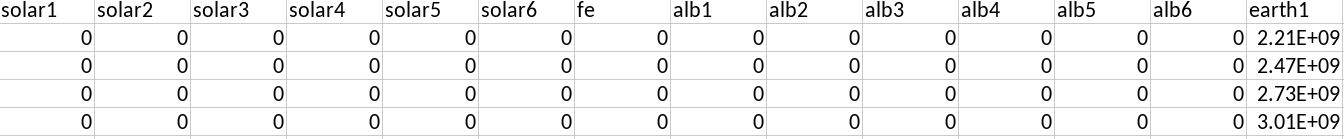
\includegraphics[width=0.8\textwidth]{fig/cleandataset.png}
\caption{Contoh dataset yang sudah disaring}
\label{fig:cleandataset}
\end{center}
\end{figure}


\section{Pelatihan dan Pengujian Model}

Dataset yang sudah disaring kemudian dibagi menjadi set latihan
(\textit{training}) dan ujian (\textit{test}) dengan menggunakan modul
Scikit-learn. Pemodelan pada karya tulis ini menggunakan rasio jumlah data
pelatihan dibanding pengujian sebesar 0.7:0.3 serta pengaturan \textit{seed
number} 0. Tabel \ref{table:dataset} memuat detail jumlah dataset yang
digunakan dalam pemodelan untuk kedua periode observasi.

\begin{table}[!ht]
\begin{center}
\caption{Detail jumlah dataset model \textit{machine learning}}
\label{table:dataset}
\begin{tabular}{|c|cc|}
\hline
\multirow{2}{*}{Tanggal} & \multicolumn{2}{c|}{Dataset}                 \\ \cline{2-3} 
                         & \multicolumn{1}{c|}{Set latihan} & Set ujian \\ \hline
19 Mei 2018              & \multicolumn{1}{c|}{201}         & 87        \\ \hline
20 Mei 2018              & \multicolumn{1}{c|}{180}         & 78        \\ \hline
\end{tabular}
\end{center}
\vspace{-5mm}
\end{table}

Pelatihan dan pengujian model dipisah per tanggal observasi karena pada
Persamaan \ref{eq:lineq} koefisien $c_a$ mengandung nilai sudut bidang orbit
satelit terhadap Matahari $\beta$ yang dianggap konstan selama 1 periode
observasi. Nilai $\beta$ bergantung pada posisi Bumi relatif terhadap Matahari.
Dengan kata lain, nilai $\beta$ berubah seiring dengan pergantian hari
sepanjang tahun akibat revolusi Bumi mengitari Matahari \cite{m2019}.
